\documentclass[a4paper,12pt]{article}
\usepackage{amsmath}
\usepackage{graphicx}
\usepackage{hyperref}
\usepackage{mathptmx}
\usepackage[brazil]{babel}

\title{Lista 5 - Cloud Computing}
\author{Breno Fernandes - 01169313}
\date{\today}

\begin{document}

\maketitle

\section*{Questão 1}
Uma rede tem largura de banda de 10 Mbps e é capaz de transmitir 12.000 pacotes por minuto, com cada pacote contendo 10.000 bits. Para calcular o throughput real da rede, precisamos considerar tanto a largura de banda quanto a taxa de transmissão dos pacotes.

\subsection*{Cálculo do Throughput}
\begin{itemize}
    \item Largura de banda: 10 Mbps = \( 10 \times 10^6 \) bits por segundo.
    \item Número de pacotes por minuto: 12.000 pacotes/minuto.
    \item Cada pacote contém: 10.000 bits.
\end{itemize}

Convertendo a taxa de pacotes para segundos:
\[
\text{Taxa de pacotes por segundo} = \frac{12000}{60} = 200 \text{ pacotes/segundo}
\]

O throughput é dado pelo produto da taxa de pacotes e o tamanho de cada pacote:
\[
\text{Throughput} = 200 \text{ pacotes/s} \times 10.000 \text{ bits/pct} = 2.000.000 \text{ bits/s} = 2 \text{ Mbps}
\]

Portanto, o throughput real da rede é de 2 Mbps.

\subsection*{Conclusão}
Embora a largura de banda nominal da rede seja de 10 Mbps, o throughput real observado é de apenas 2 Mbps. Isso indica que a rede opera com um aproveitamento de apenas 20\% da largura de banda máxima, possivelmente devido a fatores como overhead de protocolo ou limitações no processamento de pacotes.

\section*{Questão 2}
Os quatro componentes da latência que afetam o desempenho de uma aplicação em nuvem são::

\begin{itemize}
    \item \textbf{Tempo de Propagação:} É o tempo que um sinal leva para viajar de um ponto a outro. Em aplicações em nuvem, isso pode ser crítico, especialmente se os servidores estiverem localizados em regiões geográficas distantes. Quanto maior a distância física entre o cliente e o servidor, maior será o tempo de propagação, resultando em tempos de resposta mais lentos.

    \item \textbf{Tempo de Transmissão:} Refere-se ao tempo necessário para enviar todos os bits de um pacote. Em redes com alta largura de banda, esse tempo é menor e menos impactante, mas em conexões mais lentas, o tempo de transmissão pode se tornar significativo, afetando a experiência do usuário, especialmente em transferências de grandes volumes de dados.

    \item \textbf{Tempo de Fila:} Esse é o tempo que um pacote passa em uma fila antes de ser transmitido. Em momentos de congestionamento da rede, o tempo de fila pode aumentar consideravelmente, causando uma maior latência geral. Em serviços em nuvem, isso pode ocorrer em situações de alta demanda, especialmente em servidores que gerenciam múltiplas requisições simultâneas.

    \item \textbf{Tempo de Processamento:} O tempo que um dispositivo leva para processar o pacote, incluindo a verificação de erros e o roteamento. Esse componente pode ser crítico em servidores de alta carga e impacta diretamente a eficiência do sistema, podendo resultar em atrasos significativos caso o servidor esteja sobrecarregado.
\end{itemize}

\subsection*{Cenário Prático}
Um cenário onde a latência pode ser crítica é em aplicações de jogos online. A comunicação em tempo real entre jogadores requer tempos de resposta muito baixos; qualquer atraso perceptível pode comprometer a experiência do usuário, resultando em jogabilidade prejudicada e frustração. Por exemplo, em um jogo de tiro em primeira pessoa, até mesmo um pequeno atraso na resposta aos comandos do jogador pode fazer com que ele perca ações importantes. Esse tipo de aplicação depende de uma latência mínima para garantir uma experiência de jogo fluida e responsiva.


\section*{Questão 3}
Durante uma transmissão de vídeo ao vivo em um sistema de nuvem, 3\% dos pacotes são perdidos. Isso pode impactar a qualidade da transmissão de várias maneiras:

\begin{itemize}
    \item \textbf{Interrupções na Transmissão:} A perda de pacotes pode resultar em quadros perdidos, causando "cortes" visíveis na transmissão de vídeo. Esse problema é mais perceptível em transmissões em tempo real, onde há menos tempo para recuperação de dados perdidos.
    
    \item \textbf{Degradação da Qualidade:} A compressão e a codificação podem não ser suficientes para corrigir a perda, levando a uma degradação geral da qualidade do vídeo, como pixelização, borrão ou congelamento de quadros. Esse impacto é mais evidente em vídeos de alta definição, onde a perda de pacotes afeta mais diretamente a nitidez da imagem.
\end{itemize}

\subsection*{Técnicas de Mitigação}
Para mitigar a perda de pacotes, as seguintes técnicas podem ser aplicadas:

\begin{itemize}
    \item \textbf{Redundância:} Transmitir pacotes redundantes ou utilizar técnicas de codificação que permitam a recuperação de dados perdidos. Isso garante que, mesmo com a perda de alguns pacotes, os dados essenciais possam ser reconstruídos sem impacto perceptível para o usuário.
    
    \item \textbf{Buffering:} Implementar buffers que armazenam temporariamente os dados recebidos antes da reprodução. O buffer permite que o sistema compense pequenas perdas de pacotes e flutuações na taxa de transmissão, garantindo uma reprodução mais fluida.

    \item \textbf{Protocolos de Correção de Erros:} Utilizar protocolos que incluem mecanismos de correção de erros, como o Forward Error Correction (FEC), para reconstruir pacotes perdidos. Em transmissões ao vivo, onde retransmissões podem não ser viáveis devido a restrições de tempo, o FEC é uma solução eficaz para melhorar a qualidade final da transmissão.

    \item \textbf{Ajuste Dinâmico da Qualidade (ABR - Adaptive Bitrate):} Em plataformas de streaming, essa técnica ajusta a qualidade do vídeo com base na largura de banda disponível e na taxa de perda de pacotes, garantindo que a transmissão se adapte às condições da rede\dots

  \end{itemize}

\section*{Questão 4 - Atividade Prática}

Medição e Análise de Desempenho de rede

\subsection*{Configuração dos dispositivos}

Para esse teste foram utilizados dois dispositivos, um \textbf{desktop} e um \textbf{notebook}, ambos conectados no mesmo roteador \textit{mikrotik}. No primeiro momento o notebook estava utilizando a rede sem fios, mas para fins de comparação, também executei os testes utilizando a rede cabeada.
O desktop possui uma placa de rede de 2.5gbps, enquanto o notebook possui uma conexão rj-45 1gbps. 
Apenas o notebook possui rede wi-fi, que teoricamente também pode alcançar velocidades de até 1gbps, mas como pode-se constatar nos resultados do iperf3 não é bem o que acontece na prática. 


\subsection*{Início dos testes}
A ferramenta \textbf{iperf3} foi instalada em embos os computadores para efetuar a medição do desempenho.

Também realizei testes de \textit{ping} para determinar a latência entre os dois hosts.
\begin{figure}[h!]
  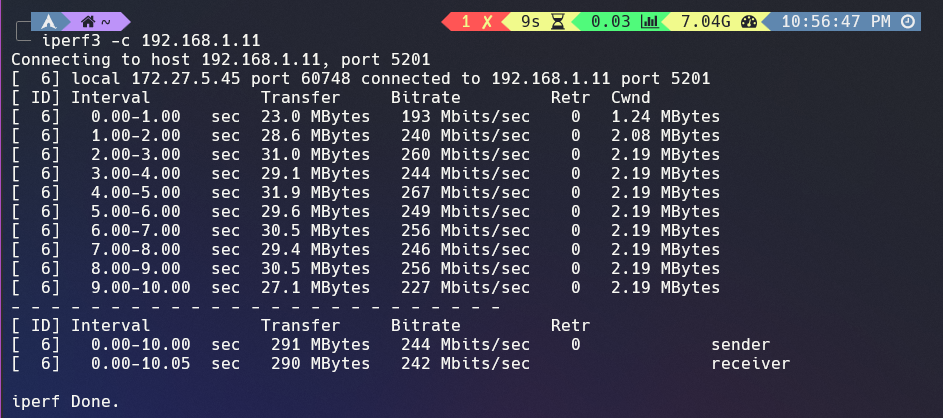
\includegraphics[width=1.0\textwidth]{img/iperf3-wifi.png}
  \caption{Teste com iperf3 utilizando rede sem fio.}
\end{figure}

\begin{figure}
  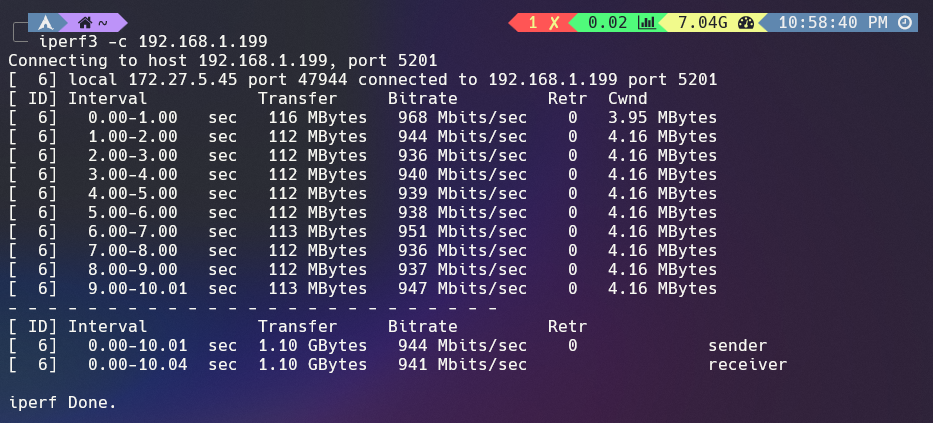
\includegraphics[width=1.0\textwidth]{img/iperf3-utp.png}
  \caption{Teste com iperf3 utilizando rede cabeada.}

  \centering
  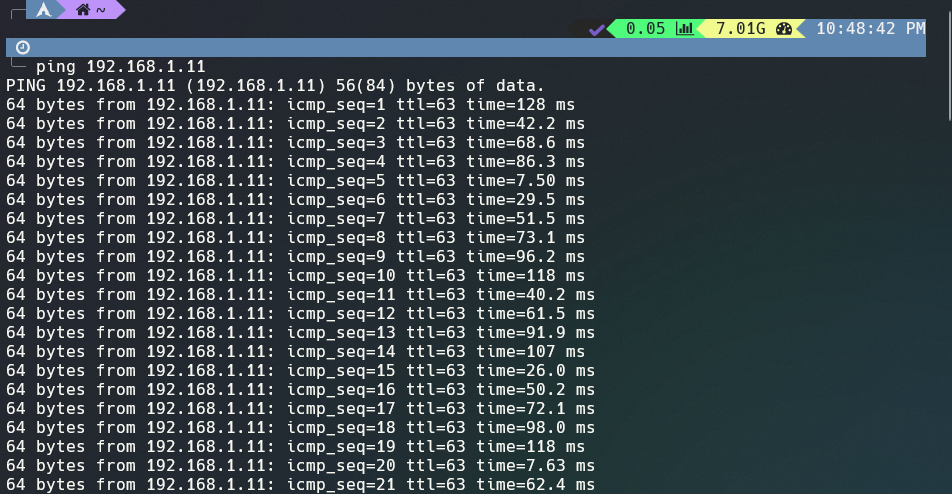
\includegraphics[width=1.0\textwidth]{img/latencia-wifi.png}
  \caption{Latência entre os hosts utilizando rede sem fio.}

  \centering
  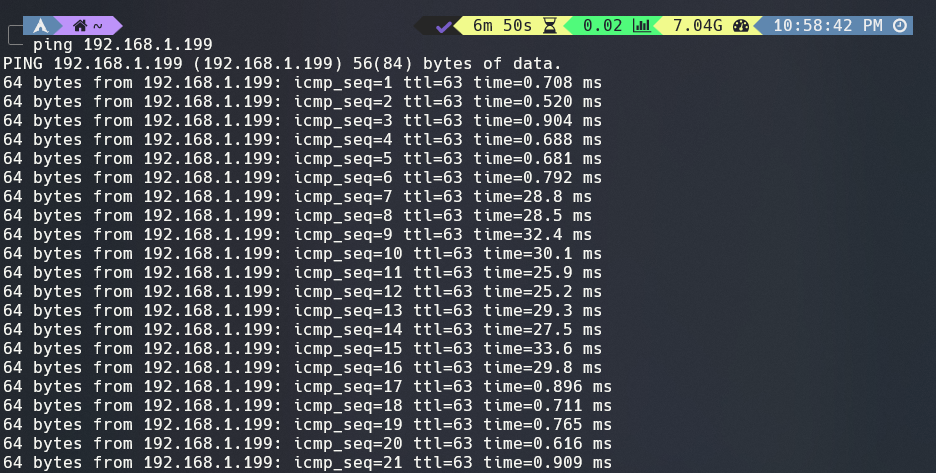
\includegraphics[width=1.0\textwidth]{img/latencia-cabo.png}
  \caption{Latência entre os hosts utilizando rede cabeada.}
\end{figure}
\break
\section*{O que é Jitter}

\textbf{Jitter} é a variação no tempo de atraso entre a transmissão de pacotes em uma rede. Em uma conexão ideal, os pacotes são entregues em intervalos regulares. No entanto, em redes reais, esses intervalos podem variar devido a fatores como congestionamento, processamento e enfileiramento nos dispositivos de rede. 
\subsection*{Como calcular o jitter}
Para calcular o jitter entre pacotes, é possível usar a diferença entre os tempos de atraso consecutivos. Por exemplo, se temos três pacotes com tempos de atraso \(d_1\), \(d_2\) e \(d_3\):

\begin{itemize}
    \item Calcule a diferença entre os tempos de atraso consecutivos: \((d_2 - d_1)\) e \((d_3 - d_2)\).
    \item Encontre a média das diferenças absolutas entre esses tempos.
\end{itemize}

Assim, o jitter médio é uma média das variações entre os tempos de entrega dos pacotes ao longo do tempo.

\section*{Cálculo do Jitter com Dados de Ping}

É possível calcular o jitter usando os dados obtidos de um teste de \texttt{ping}. Os resultados do \texttt{ping} fornecem os tempos de ida e volta de cada pacote enviado, o que permite calcular o jitter como a variação nos tempos entre pacotes consecutivos.

\subsection*{Passos para calcular o jitter com dados do ping}
\begin{enumerate}
    \item Coletar o \texttt{ping} e anotando o tempo de cada pacote, que é exibido em ms no retorno de cada resposta.
    
    \item \textbf{Calcular a diferença entre os tempos consecutivos:} Para cada par de tempos de RTT consecutivos \( RTT_n \) e \( RTT_{n-1} \), calcule a diferença absoluta:
    \[
    \text{Diferença}_n = | RTT_n - RTT_{n-1} |
    \]

    \item \textbf{Jitter médio:} Tirando a média das diferenças calculadas dá para se obter o jitter médio:
    \[
    \text{Jitter Médio} = \frac{\sum_{n=2}^{N} |\text{RTT}_n - \text{RTT}_{n-1}|}{N - 1}
    \]
    onde \( N \) é o número total de pacotes.
\end{enumerate}

Esse cálculo fornece o valor médio de jitter e pode dar uma boa indicação da variação na latência da rede, especialmente útil para analisar a estabilidade da conexão.

\subsection*{Jitter médio da rede sem fio}

Dado os tempos de ida e volta em milissegundos:
\[
128, \ 42.2, \ 68.6, \ 86.3, \ 7.5, \ 29.5, \ 51.5, \ 73.1, \ 96.2, \ 118, \ 40.2, \ 61.5, \ 91.9, \ 107, \ 26.8, \ 50.2, \ 72.1, \ 98.0, \ 118, \ 7.63, \ 62.4
\]

Calcula-se as diferenças absolutas entre tempos consecutivos:
\[
\begin{align*}
|128 - 42.2| &= 85.8 \\
|42.2 - 68.6| &= 26.4 \\
|68.6 - 86.3| &= 17.7 \\
|86.3 - 7.5| &= 78.8 \\
|7.5 - 29.5| &= 22.0 \\
|29.5 - 51.5| &= 22.0 \\
|51.5 - 73.1| &= 21.6 \\
|73.1 - 96.2| &= 23.1 \\
|96.2 - 118| &= 21.8 \\
|118 - 40.2| &= 77.8 \\
|40.2 - 61.5| &= 21.3 \\
|61.5 - 91.9| &= 30.4 \\
|91.9 - 107| &= 15.1 \\
|107 - 26.8| &= 80.2 \\
|26.8 - 50.2| &= 23.4 \\
|50.2 - 72.1| &= 21.9 \\
|72.1 - 98.0| &= 25.9 \\
|98.0 - 118| &= 20.0 \\
|118 - 7.63| &= 110.37 \\
|7.63 - 62.4| &= 54.77 \\
\end{align*}
\]

Somando essas diferenças e dividindo pelo número de diferenças, obtem-se o jitter médio:
\[
\text{Jitter Médio} = \frac{\sum_{n=2}^{21} |\text{RTT}_n - \text{RTT}_{n-1}|}{20} = \frac{800.34}{20} \approx 40.02 \text{ ms}
\]

Portanto, o jitter médio para o teste com o notebook na rede sem fio é de aproximadamente \( 40.02 \) ms.

\subsection*{Jitter médio rede cabeada}

Dado os pings em ms:
\[
0.708, \ 0.520, \ 0.904, \ 0.688, \ 0.681, \ 0.792, \ 2.8, \ 2.5, \ 32.4, \ 30.1,
\ 25.9, \ 27.5, \ 33.6, \ 29.8, \ 0.986, \ 0.711, \ 0.765, \ 0.616, \ 0.909
\]

Calcula-se as diferenças:
\[
\begin{align*}
|0.708 - 0.520| &= 0.188 \\
|0.520 - 0.904| &= 0.384 \\
|0.904 - 0.688| &= 0.216 \\
|0.688 - 0.681| &= 0.007 \\
|0.681 - 0.792| &= 0.111 \\
|0.792 - 2.8| &= 2.008 \\
|2.8 - 2.5| &= 0.300 \\
|2.5 - 32.4| &= 29.900 \\
|32.4 - 30.1| &= 2.300 \\
|30.1 - 25.9| &= 4.200 \\
|25.9 - 27.5| &= 1.600 \\
|27.5 - 33.6| &= 6.100 \\
|33.6 - 29.8| &= 3.800 \\
|29.8 - 0.986| &= 28.814 \\
|0.986 - 0.711| &= 0.275 \\
|0.711 - 0.765| &= 0.054 \\
|0.765 - 0.616| &= 0.149 \\
|0.616 - 0.909| &= 0.293 \\
\end{align*}
\]

Somando essas diferenças e dividindo pelo número de diferenças, obtem-se o jitter médio:
\[
\text{Jitter Médio} = \frac{\sum_{n=2}^{18} |\text{RTT}_n - \text{RTT}_{n-1}|}{17} = \frac{75.639}{17} \approx 4.48 \text{ ms}
\]

Portanto, o jitter médio na ocasião onde o notebook está conectado na rede cabeada é de aproximadamente \( 4.48 \) ms.

\end{document}
